\documentclass[10pt]{article}
\usepackage[margin=1.5cm]{geometry}
\usepackage{multicol}
\usepackage{caption} % or \usepackage{capt-of}
\usepackage{amsmath, amssymb}
\usepackage{bm}
\usepackage{titlesec}
\usepackage{graphicx}
\usepackage[most]{tcolorbox}

% Define a compact style for cheat sheet boxes (optional)
\tcbset{
  cheatbox/.style={
    colback=gray!10,       % light gray background
    colframe=gray!60,      % darker border
    boxrule=0.5pt,
    arc=3pt,               % rounded corners
    left=6pt, right=6pt, top=4pt, bottom=4pt,
    enhanced,
  }
}

%Compact style
\setlength{\parindent}{0pt}
\setlength{\parskip}{0pt}
\setlength{\columnsep}{12pt}

\DeclareMathOperator{\cov}{Cov}

% Compact section formatting
\titleformat{\section}{\large\bfseries}{}{0pt}{}
\titleformat{\subsection}{\normalsize\bfseries}{}{0pt}{}
\titleformat{\paragraph}[runin]{\normalsize\bfseries}{}{0pt}{}[.]

% \setlength{\parindent}{0pt}
% \setlength{\parskip}{4pt}
% \pagestyle{empty}

\begin{document}
\begin{center}
    {\Large \textbf{Error Propagation and Bootstrapping Cheatsheet}}\\[4pt]
\end{center}
Bootstrapping is used to estimate uncertainty when the sampling distribution is unknown or hard to derive, especially for small samples or complex statistics.
\begin{multicols*}{2}
\raggedcolumns

\section*{Variance and Standard Error}

\noindent
\textbf{Variance}
For \( N \) observations of variable \( x_i \),
\(\mathbf{x}_i = \{ x_{i,1}, x_{i,2}, \ldots, x_{i,N} \}\), with mean \(\bar{x}_i\):
\[
\sigma_i^2 = \frac{1}{N - 1} \sum_{n=1}^{N} (x_{i,n} - \bar{x}_i)^2
\]
measures the spread of \( x_i \) around its mean.



\textbf{Standard Error of the Mean (SEM)}
\begin{equation}
\mathrm{SEM}_{i} = \frac{\sigma_i}{\sqrt{N}}
\end{equation}
The standard error quantifies the uncertainty in the mean's estimate. As \( N \) increases, the standard error decreases.

% \paragraph{Relation Between Variance and Standard Error}
% \begin{equation}
% \mathrm{Var}(\bar{x}) = \frac{\mathrm{Var}(x)}{n}
% \quad \Rightarrow \quad
% \mathrm{SE}_{\bar{x}} = \sqrt{\mathrm{Var}(\bar{x})} = \frac{\sqrt{\mathrm{Var}(x)}}{\sqrt{n}} = \frac{s}{\sqrt{n}}
% \end{equation}
\section*{Error propagation Formula}


For a function 
\[
y = f(\mu_1, \mu_2, \ldots, \mu_m)
\]
where $\mu_i$ are measured values, e.g. means, with variances $\sigma_{i}^2$ and covariances $\Sigma_{ij}$. Propagated error is given by:
\[
\sigma_y^2 =
\sum_{i=1}^{m}
\left(
\frac{\partial f}{\partial \mu_i}
\right)^2
\sigma_{i}^2
+ 2 \sum_{i<j}
\frac{\partial f}{\partial \mu_i}
\frac{\partial f}{\partial \mu_j}
\Sigma_{ij}
\]
\textbf{Common formulas}\\[3pt]
Addition/Subtraction
\[
y = \mu_1 \pm \mu_2
\quad \Rightarrow \quad
\sigma_y^2 = \sigma_{1}^2 + \sigma_{2}^2
\]
Multiplication/Division
\[
y = \mu_1^{a_1} \mu_2^{a_2} \cdots \mu_m^{a_m}
\quad \Rightarrow \quad
\left( \frac{\sigma_y}{y} \right)^2 =
\sum_{i=1}^{m}
a_i^2
\left(
\frac{\sigma_{i}}{\mu_i}
\right)^2
\]


\paragraph{Example}
\[
y = \frac{AB}{C^2}
\]

\[
\left(\frac{\sigma_y}{y}\right)^2 =
\left(\frac{\sigma_A}{A}\right)^2 +
\left(\frac{\sigma_B}{B}\right)^2 +
\left(2\frac{\sigma_C}{C}\right)^2
\]

If \(A=2.50\pm0.03\), \(B=1.20\pm0.02\), \(C=3.00\pm0.05\):
$y = 0.333 \pm 0.013$

\textbf{Practical Tips}

\begin{itemize}
  \item Only use when $y\gg \sigma_{y}$ or $f$ is linear otherwise this formula
  does not hold! e.g. $f(x)=e^{x^2} \;\text{with} \;x,\sigma_x>1$
    \item For nonlinear models or large uncertainties, use \textbf{\textit{Monte Carlo}} propagation:
  simulate many draws of \(\{x_i\}\) from their distributions, compute \(f\) each time, and take the standard deviation of results.
  \item Report results as \( y \pm \sigma_y \) (68\% confidence) unless otherwise stated.
\end{itemize}
\columnbreak
\begin{minipage}{\columnwidth}
\centering
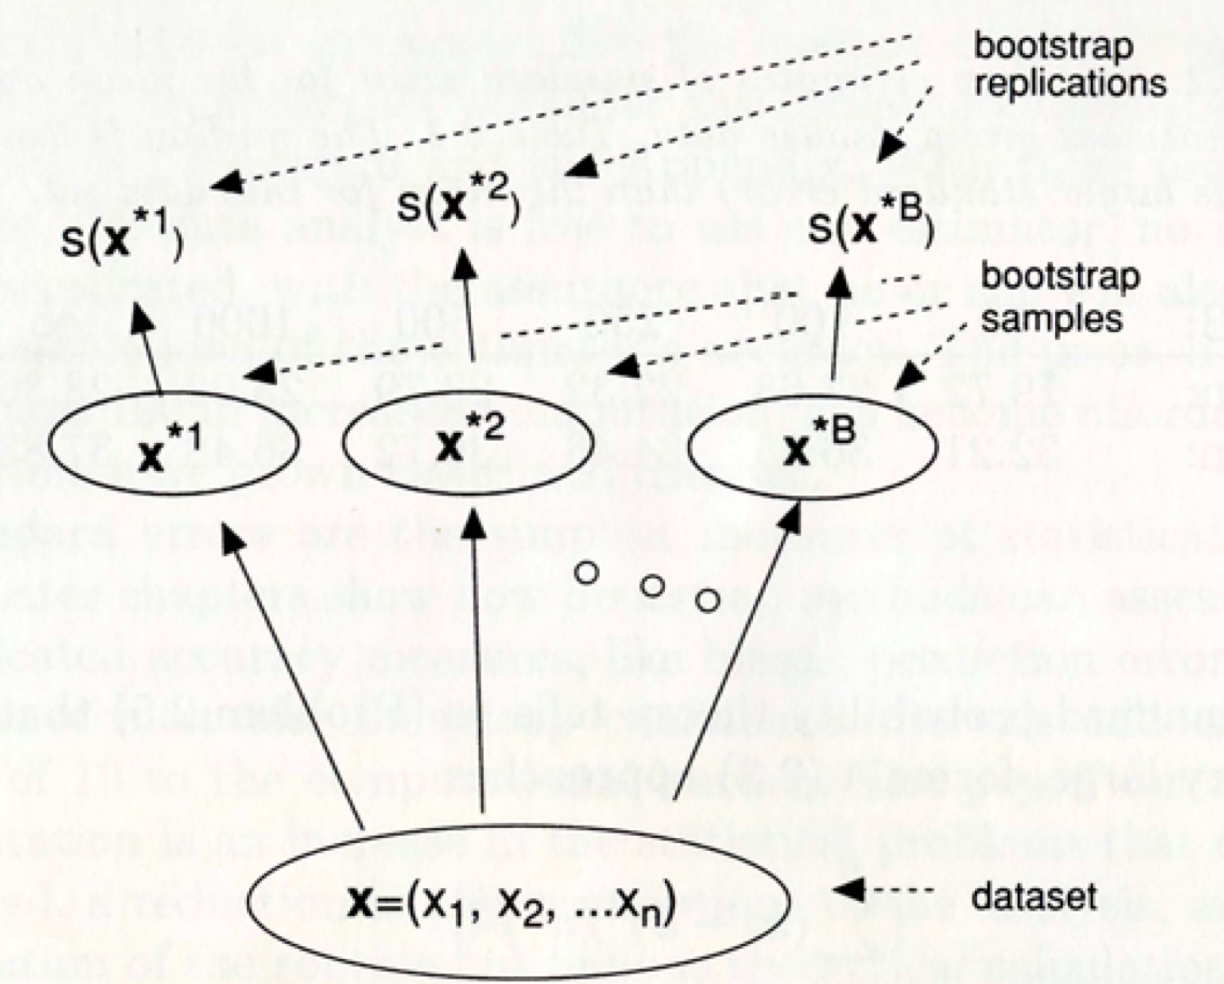
\includegraphics[width=.9\linewidth]{bootstrap_diagram.png}
\captionof{figure}{Bootstrapping schematic}
\end{minipage}

\begin{tcolorbox}[cheatbox]
\section*{Bootstrap Procedure}
\begin{enumerate}
    \item Decide on what measure/statistic/function \( s(\mathbf{x}) \) to compute from dataset \( \mathbf{x} \).
    \item Collect \( N \) data points \( x_i \) to make dataset \( \mathbf{x} \).
    \item Create \( B \) bootstrap sample datasets \( \mathbf{x}^{*b} \) by randomly selecting \( N \) data points \textbf{with replacement} from the original dataset.
    \item Compute measure \( s(\mathbf{x}^{*b}) \) on each sample dataset.
    \item Calculate standard error or confidence error 
    \[
    \mathrm{SEM}_s^2 = \frac{1}{B - 1} \sum_{b=1}^{B} (s(\mathbf{x}^{*b}) - \bar{s}(\mathbf{x}^*))^2
    \]
    where \( \bar{s} = B^{-1} \sum_{b=1}^B s(\mathbf{x}^{*b}) \) is the mean of all bootstrap sample statistics.
\end{enumerate}
\end{tcolorbox}

\textbf{Rules of thumb}
\begin{itemize}
    \item Data points should be \textit{representative} -- lack bias or missing points.
    \item Shoot for $N>20$. Need unique bootstrap samples.
    \item $B$ should be between 100-5000. Monte Carlo error scales as $1/\sqrt{B}$. 
    \item Check the distribution shape of $s(\bm x^{*,b})$. Does it make sense? Gaussian is good but not necessary.
    \item Statistic $s(\bm x)$ needs to be “smooth” enough — small changes in the data cause small changes in the estimate.
\end{itemize}
% \section*{Bayesian Connection (Optional)}

% Frequentist error propagation assumes one true parameter; uncertainty arises from data noise.

% Bayesian inference treats parameters as random variables:
% \[
% P(\theta | D) = \frac{P(D|\theta)\,P(\theta)}{P(D)}
% \]
% Posterior $\propto$ Likelihood × Prior

% Posterior uncertainty replaces analytic error propagation when using full probabilistic models.

\end{multicols*}
\end{document}



% \documentclass{article}
% \usepackage{graphicx} % Required for inserting images

% \title{bootstrap_cheatsheet}
% \author{Adam Lamson}
% \date{October 2025}

% \begin{document}

% \maketitle

% \section{Introduction}

% \end{document}
